\section*{1. システムの概要}

% 概要図は「プロジェクトの流れについて概説」に入れる

本節では,システムで使用するDockerおよびコンテナ技術を説明し,システムの構成について述べる.


\subsection*{1-1. Dockerコンテナ}

Dockerとは,アプリケーションとその実行に必要な環境をコンテナと呼ばれる独立した単位にパッケージ化し,
どの環境でも一貫して動作させることができるプラットフォームである.
これにより,開発から本番環境までの環境の違いによる問題を減少させることができる.

\subsection*{1-2. システム構成}

本システムは,Raspberry PiによるBLEスキャンデータを基に,
混雑度を予測して可視化するシステムである.
本システムは表\ref{tbl:コンテナ}に示す 4 つのコンテナで構成される.

\begin{table}[tb]
	\centering
	\caption{コンテナ}
	\label{tbl:コンテナ}
	\small
	\doublerulesep=0.3pt
	\begin{tabular}{cccl} \hline\hline\hline
		コンテナ & 言語 & 技術 & 内容 \\ \hline
		モデル & Python & sklearn &  データの処理・予測を行う. \\
		バックエンド & Python & Flask & API の提供,データの受信・提供を行う. \\
		フロントエンド & JavaScript & React & 混雑度の可視化を行う. \\
		データベース & SQL & MySQL & データの管理を行う. \\  \hline
	\end{tabular}
\end{table}

図\ref{fig:システム概要図}に,本システムのデータの流れを示す.

\begin{figure}[tb]
	\centering
	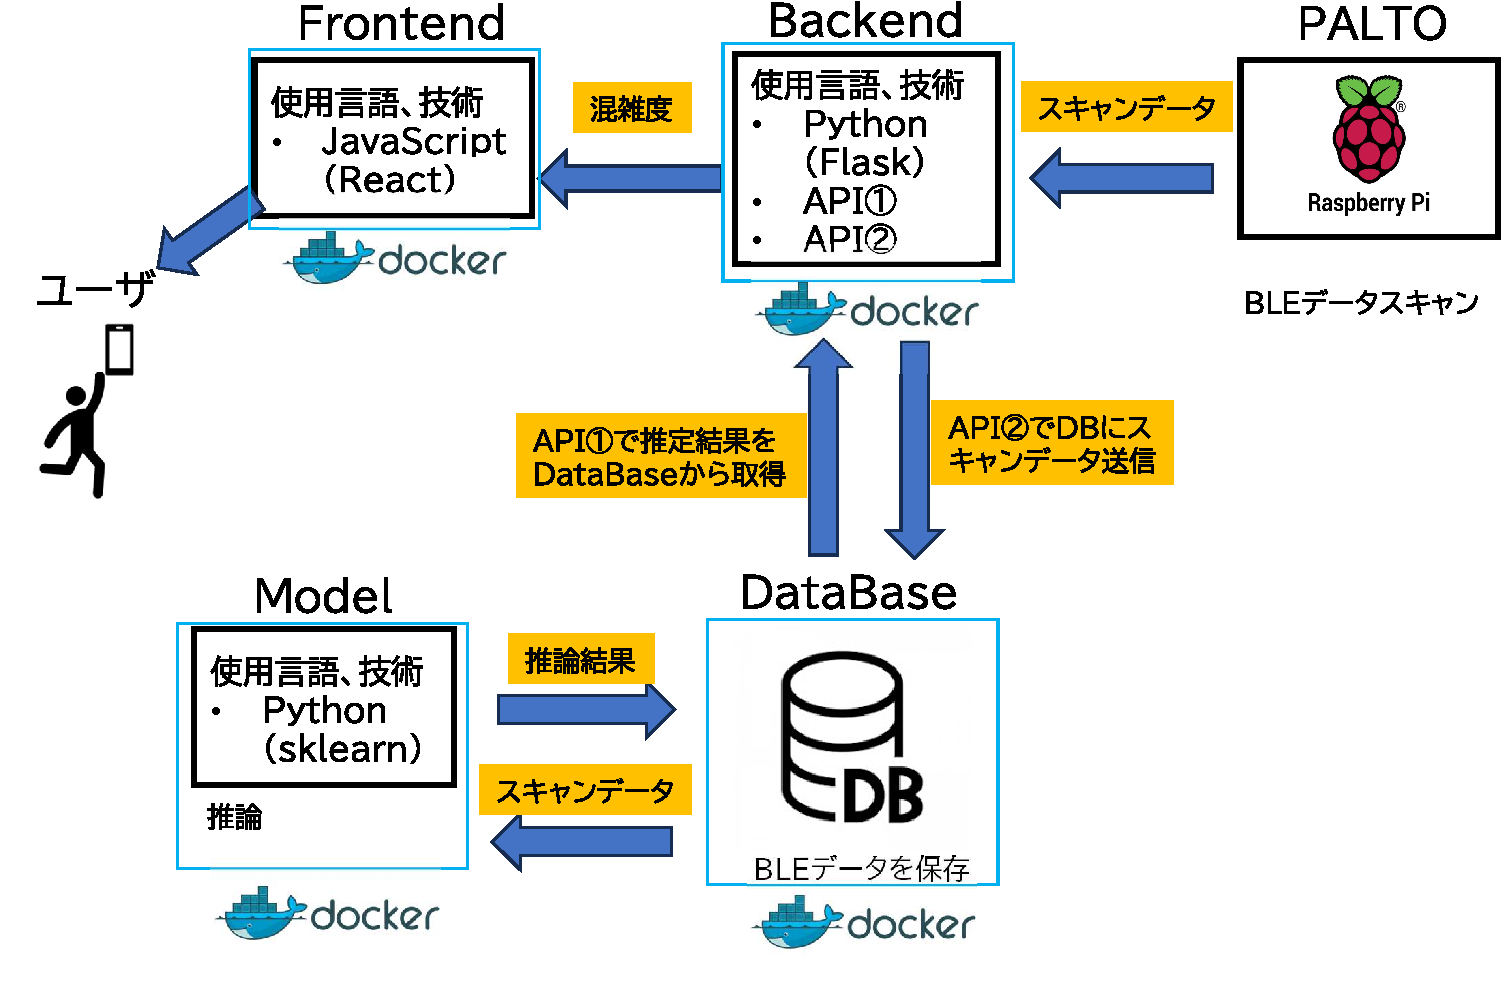
\includegraphics[width=12cm]{./outline_drawing.pdf}
	\caption{システム概要図}
	\label{fig:システム概要図}
\end{figure}

システムは,以下の流れでデータを処理する.

\begin{enumerate}
	\item データ収集 \\
	Raspberry PiがBLEスキャンを実行し,取得したデータをWi-Fi経由でサーバへ送信する.
	
	\item データ保存(API2) \\
	API2を通じて,受信したデータをデータベースコンテナに保存する.
	
	\item データ処理・予測(1分毎に実行) \\
	モデルコンテナがデータベースから取得した最新の1分間のデータから人数を予測し,データベースに保存する.
	
	\item 予測結果の取得・提供(API1) \\
	ユーザーがアプリケーションの更新ボタンを押すと,
	API1を通じてデータベースコンテナから予測結果を取得し,フロントエンドコンテナへ提供する.
	
	\item データの可視化 \\
	フロントエンドコンテナが取得したデータを可視化し,ユーザーに混雑状況を提供する.
\end{enumerate}

